\documentclass{article}
  
\usepackage{fullpage}
\usepackage{float}
\usepackage{placeins}
\usepackage{graphicx}

\begin{document}

\renewcommand\thefigure{S\arabic{figure}}
\setcounter{figure}{0}
\renewcommand\thetable{S\arabic{table}}
\setcounter{table}{0}

\title{Supplementary Material\\~\\BATCAVE: Calling somatic mutations with a tumor- and site-specific prior}

\author{
Brian K. Mannakee and
Ryan N. Gutenkunst}
\date{}

\maketitle

\begin{figure} [H]
\centering
  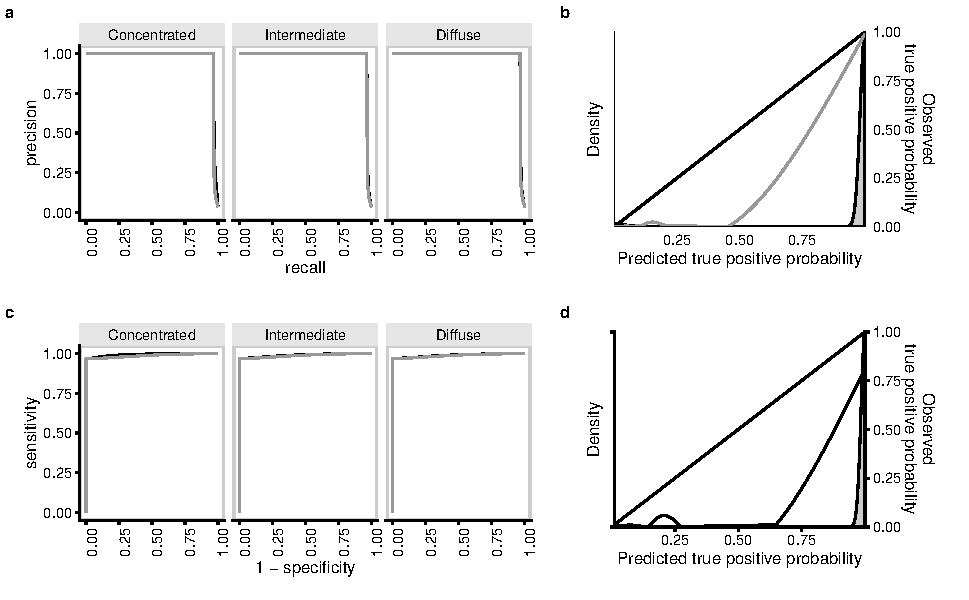
\includegraphics[width=\textwidth]{figures/fig_wgs.png}
  \caption{Variant-calling performance on  simulated 100X whole genomes. As in Fig.~4A-D, but for 100X whole genomes.}
\label{NAR-wgs_fig}
\end{figure}

\begin{figure} [H]
\centering
  \includegraphics{figures/ppv_wgs.pdf}
  \caption{Posterior probability calibration for realistic calling thresholds, for 100X whole genomes. As in Fig.~5, but for 100X whole genomes.}
\label{NAR-ppv_wgs_fig}
\end{figure}

\begin{figure} [H]
\centering
  \includegraphics[width=\textwidth]{figures/aml_sig_comp.pdf}
  \caption{Mutation profiles of A) high-confidence and B) low-confidence mutations in the AML data.}
\label{fig:AML_profiles}
\end{figure}


\begin{table*}[h]
  \caption{Sample summary for Shi et al. (2018).   }
 
 \centering
  \label{table:01}%
  \begin{tabular}{l|c|c}
  Sample & Purity estimate (\%) & Mutation rate estimate 

  \\
  \hline
  Case 1 biorep A & 53.8 & 9.3e-7 
  \\
  Case 1 biorep B & 46.3 & 8.4e-7 
  \\
  Case 1 biorep C & 26.0 & 1.0e-6 
  \\
  Case 2 biorep A & 40.0 & 1.1e-6 
  \\
  Case 2 biorep B & 32.3 & 1.0e-7 
  \\
  Case 2 biorep C & 40$^*$ & 1.0e-6
  \\
  Case 3 biorep A & 56.4 & 8.7e-7
  \\
  Case 3 biorep B & 72.8 & 7.4e-7 
  \\
  Case 3 biorep C & 64.9 & 4.3e-7 
  \\
  Case 4 biorep A & 60.4 & 8.8e-7 
  \\
  Case 4 biorep B & 61.7 & 7.9e-7 
  \\
  Case 4 biorep C & 57.6 & 8.1e-7 
  \\
  Case 5 biorep A & 78.7 & 5.7e-7 
  \\
  Case 5 biorep B & 76.7 & 5.8e-7 
  \\
  Case 5 biorep C & 80.8 & 1.8e-7 
  \\
  Case 6 biorep A & 47.8 & 2.8e-7 
  \\
  Case 6 biorep B & 49.4 & 4.1e-7 
  \\
  Case 6 biorep C & 52.9 & 4.4e-7 
  \\
  \end{tabular}

{  \small$^*$Shi et al. did not estimate purity for Case 2 biorep C. We chose 40\% purity, based on the other biological replicates from this case.}
\end{table*}

\end{document}